\providecommand{\main}{../../../..}
\documentclass[\main/dresen_thesis.tex]{subfiles}
  \renewcommand{\thisPath}{\main/chapters/monolayers/paracrystal/intro}

\begin{document}
  The long-range order of nanoparticle arrays over large areas can be quantitatively studied using x-ray and neutron scattering experiments.
  Whereas SEM is a method to obtain a local image of the structure, it leaves the possibility that the actual sample has actually great variations across the substrate, which might be overlooked.
  Also microscopy only gives an idea of the surface of the structure, while to study the vertical structure it becomes necessary to break the sample to image the cross-section.
  From grazing-incidence small-angle scattering and reflectometry experiments on the other hand the full average three dimensional information is obtained unbiased and non-invasive from a large area of the sample.

  In the following, magnetic monolayers from nanoparticles prepared by the acetylacetonate route are discussed and the used models to describe the square array structure are introduced.
  The results of the nuclear structure of the sample will then be a prerequisite to study the magnetic structure of the samples in the following section.
  The extensive study of the vertical structure is performed on monolayers prepared from the nanoparticles Ac-CoFe-C, which are also used in \refch{ch:doublelayers} to discuss double layer structures.
  The lateral structure, studied by grazing-incidence small-angle x-ray \& neutron scattering (GISAXS \& GISANS) is on the other hand performed on a second batch of nanocubes Ac-CoFe-C-2 prepared from acetylacetonates.
  The same characterization by TEM, SAXS, SANS(POL), XRD and VSM has been done for Ac-CoFe-C-2 analogue to \refsec{sec:monolayers:nanoparticle:structuralCharacterization} and can be found in \refapp{app:characterizationAcCoFeC2}.

  \begin{figure}[tb]
    \centering
    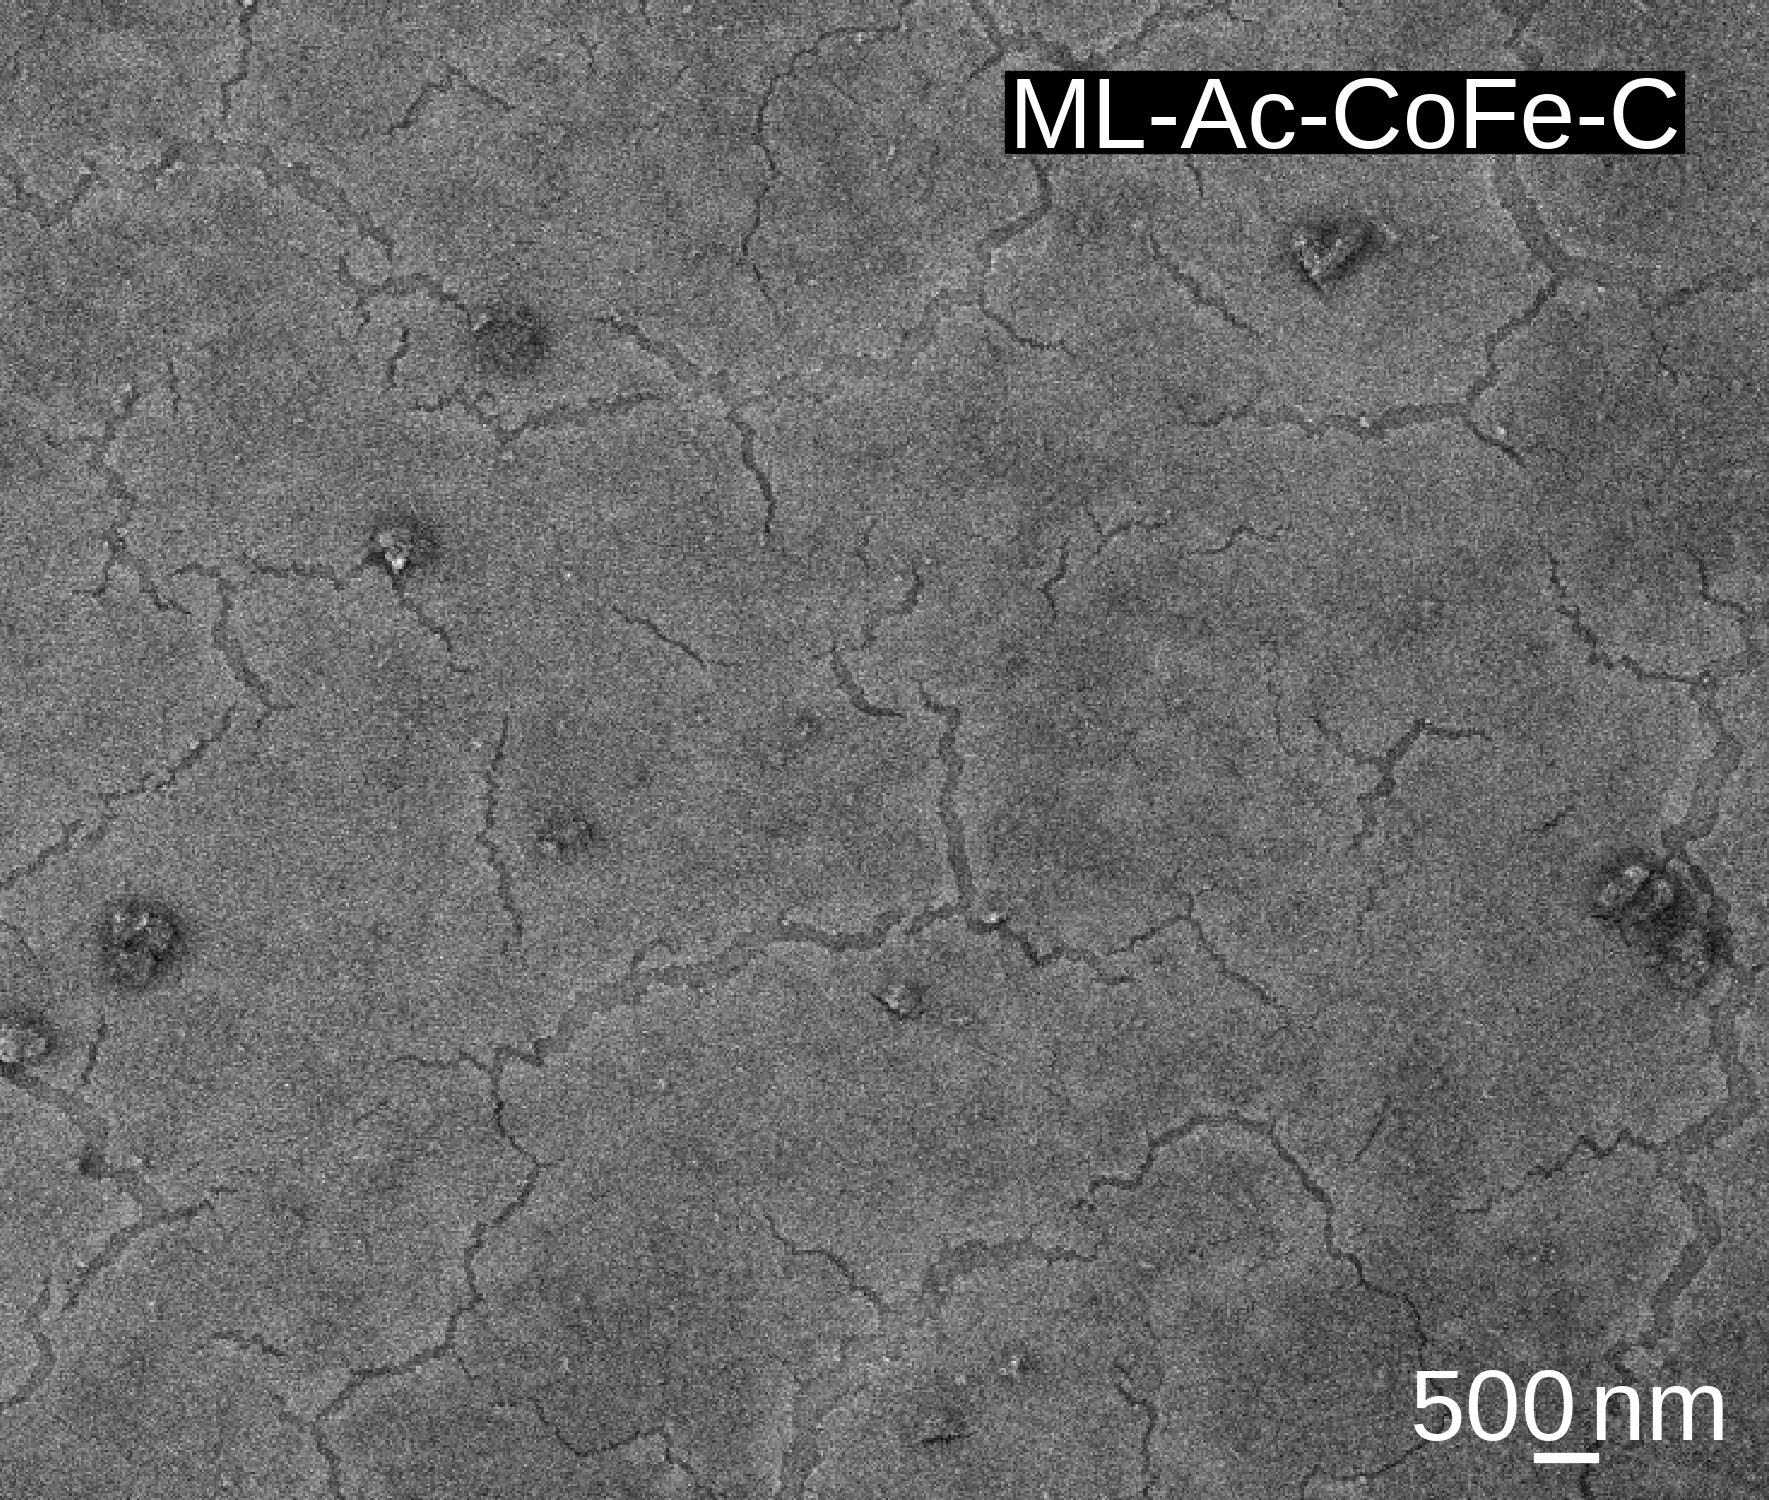
\includegraphics{monolayers_SEM_ML-Ac-CoFe-C_img1}
    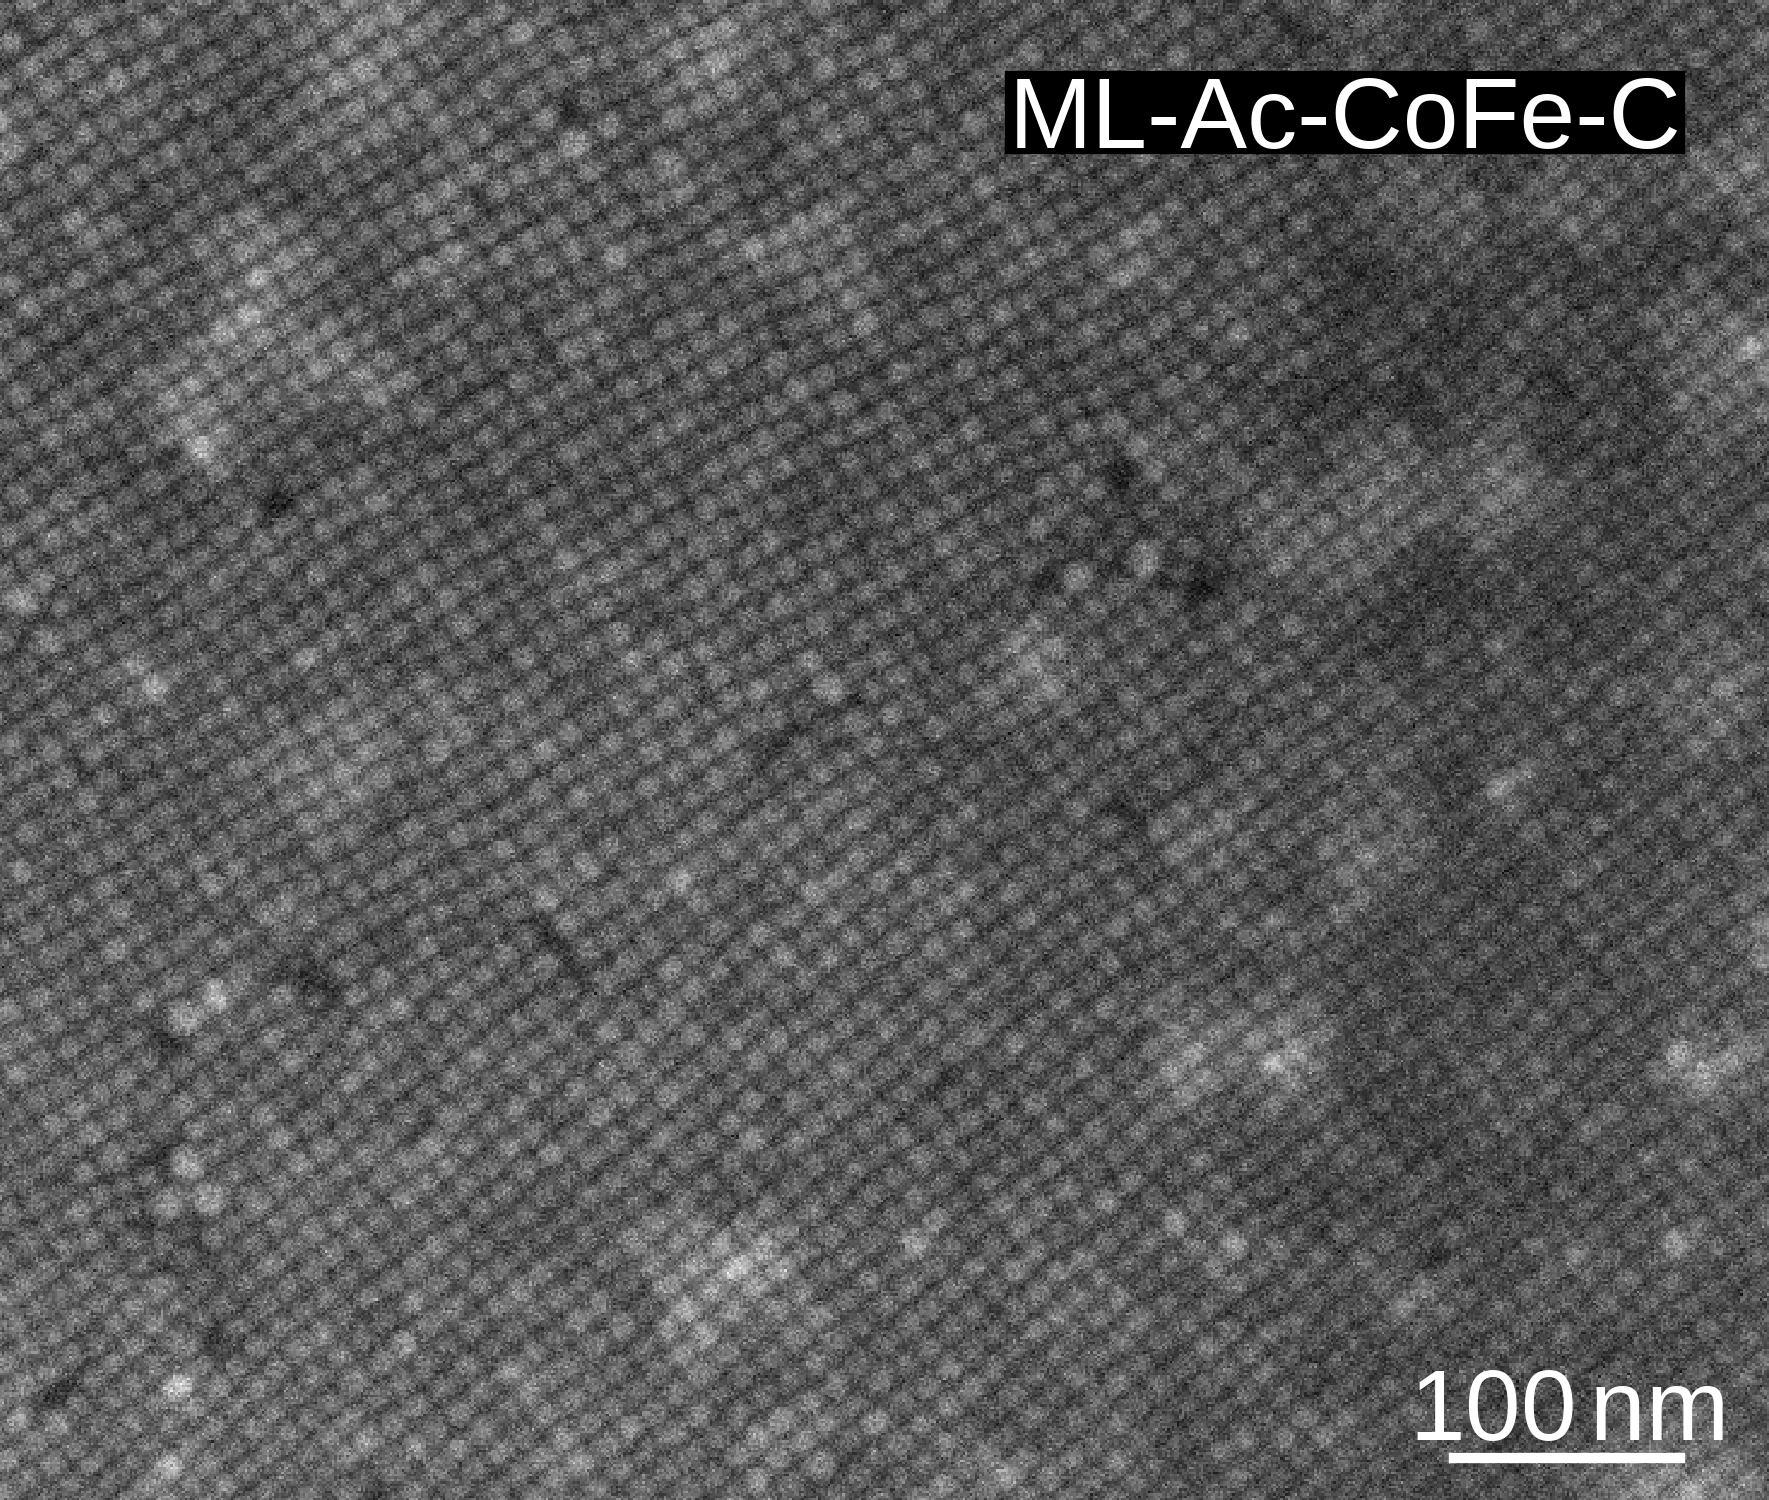
\includegraphics{monolayers_SEM_ML-Ac-CoFe-C_img2}
    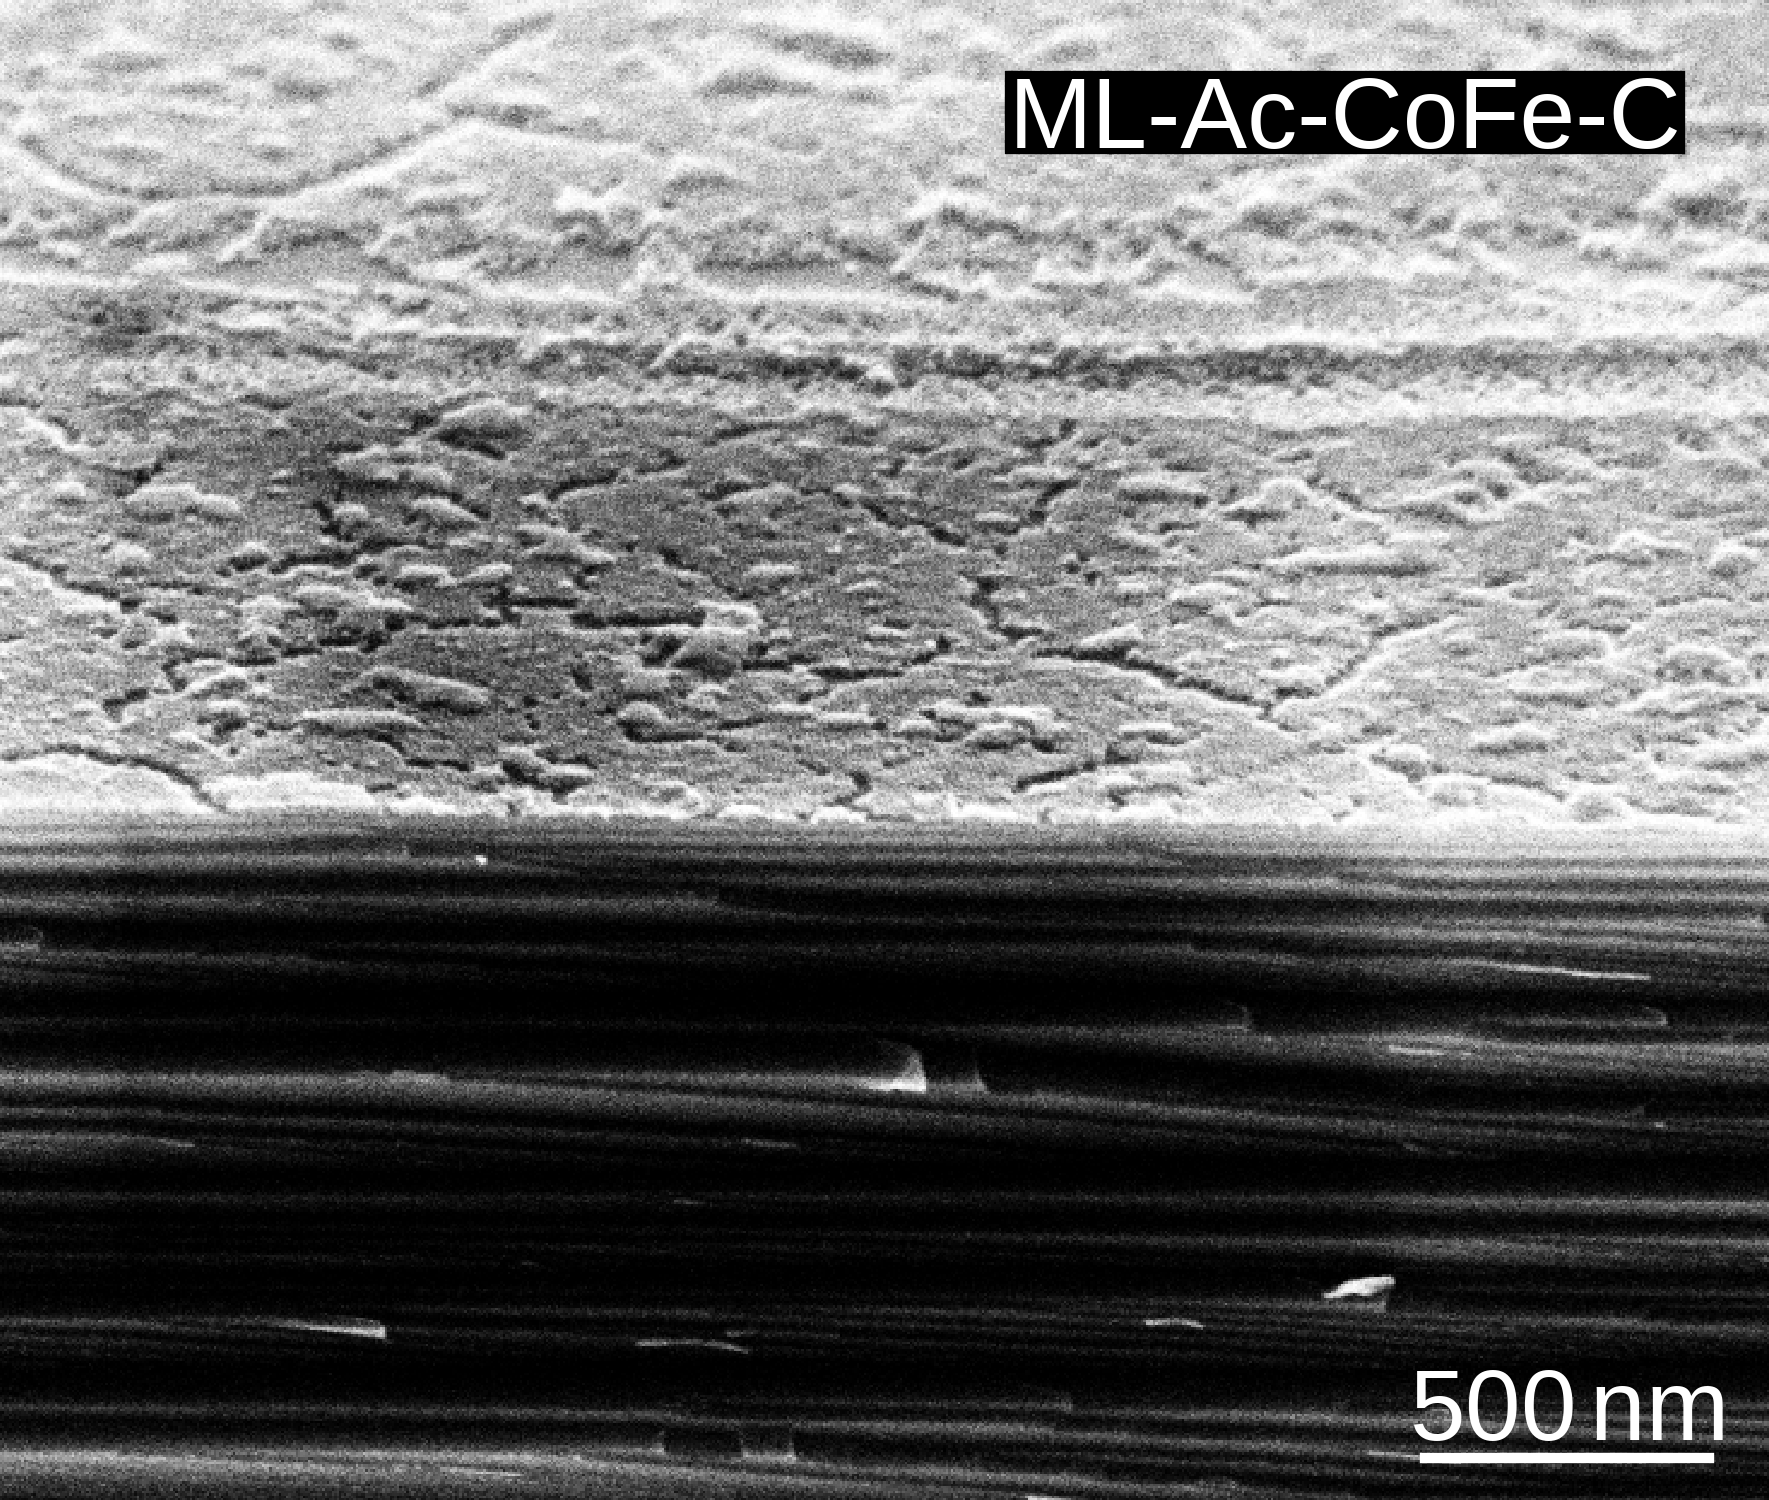
\includegraphics{monolayers_SEM_ML-Ac-CoFe-C_img3}
    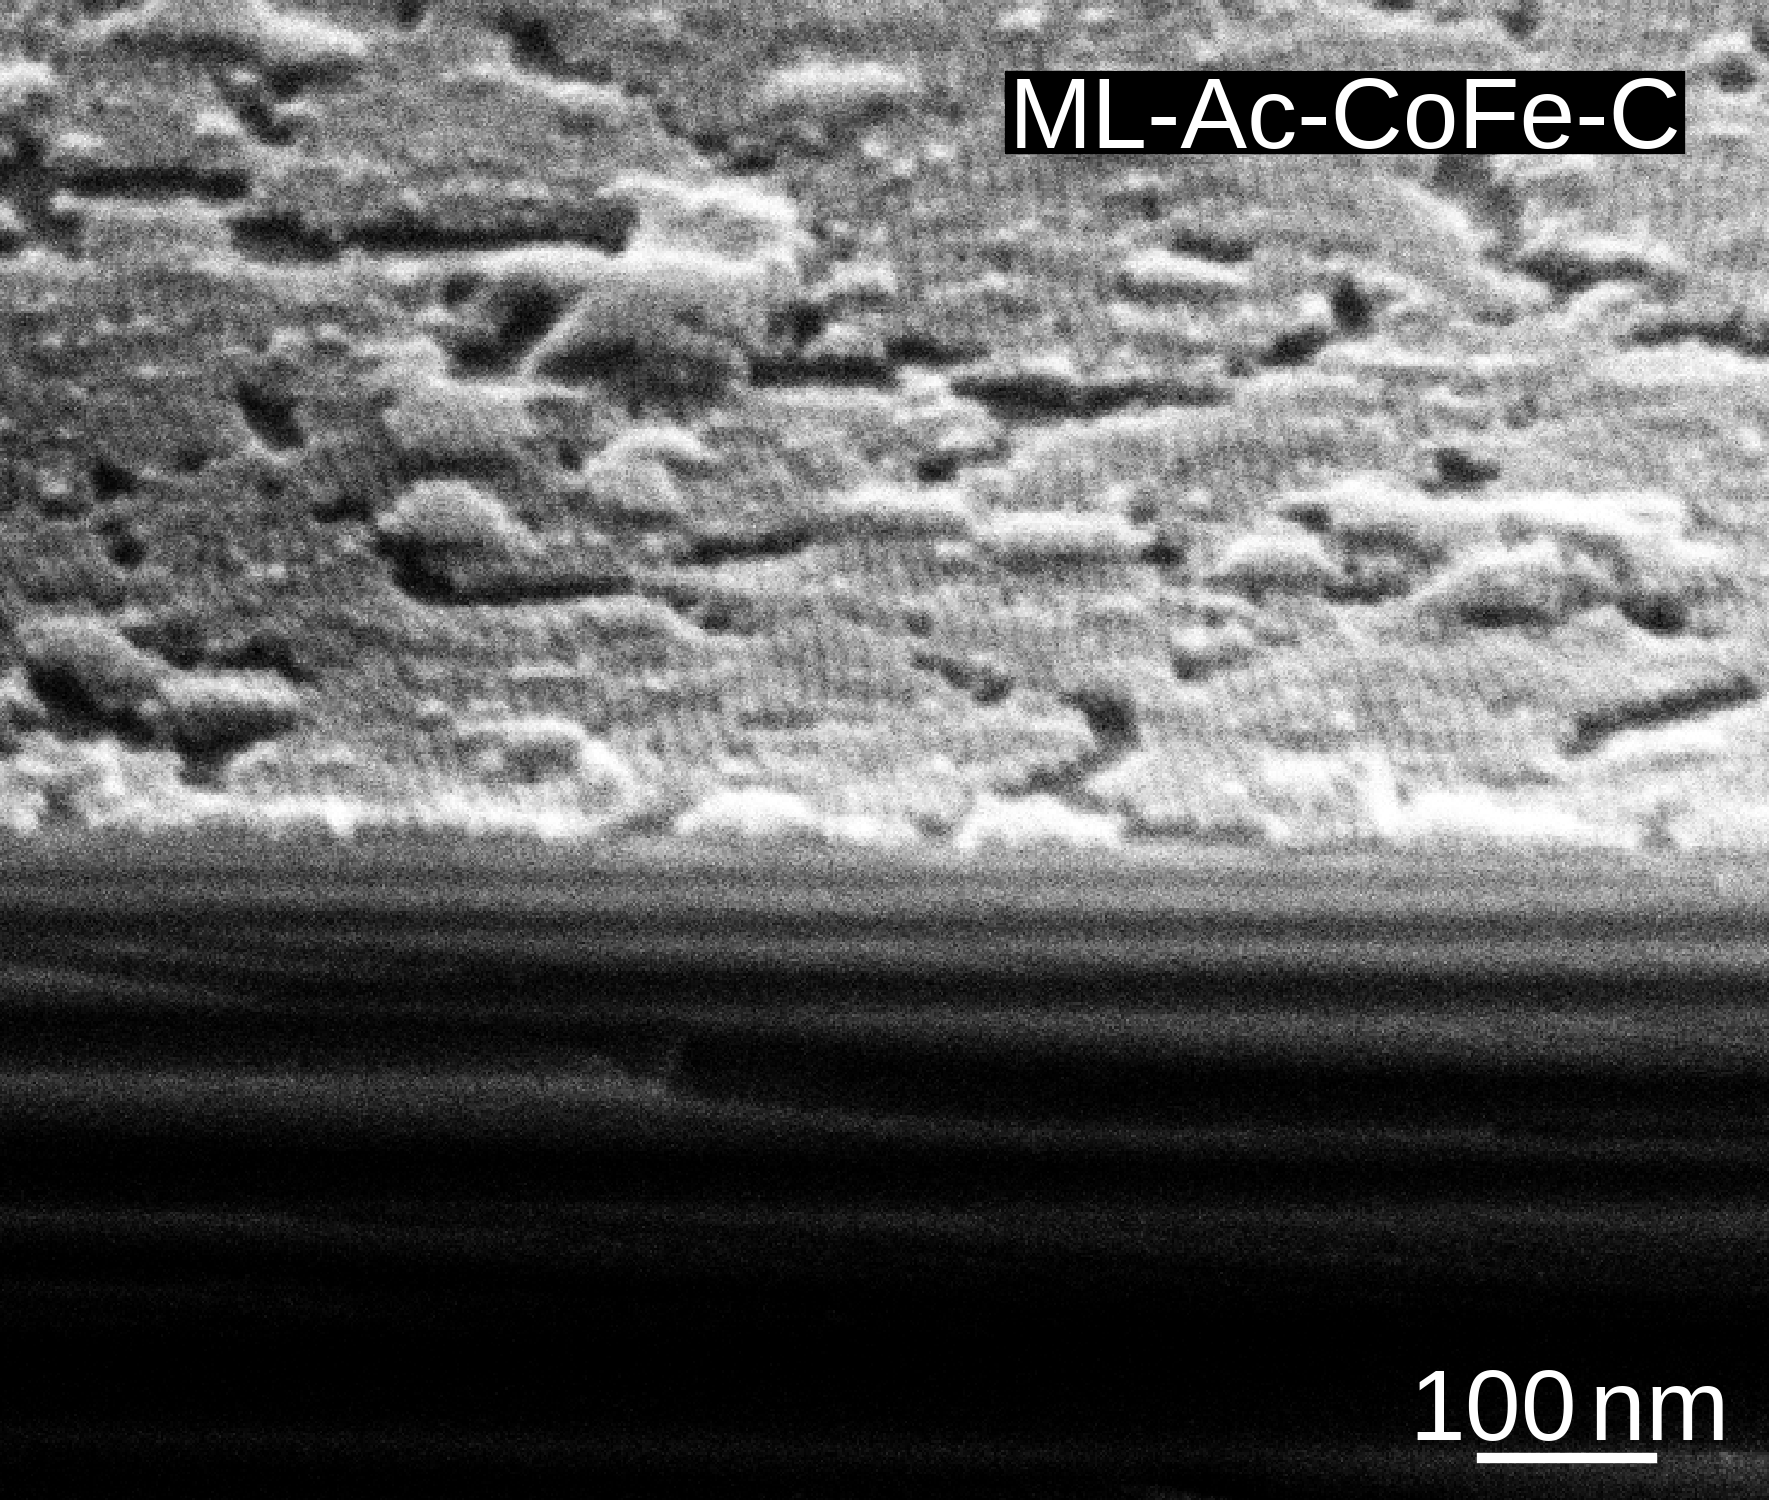
\includegraphics{monolayers_SEM_ML-Ac-CoFe-C_img4}
    \caption{\label{fig:monolayers:structure:semImagesMLACCoFeC}SEM micrographs of a monolayer prepared from Ac-CoFe-C used for the study of the vertical structure of monolayers prepared by the drop casting method.}
  \end{figure}

  \begin{figure}[tb]
    \centering
    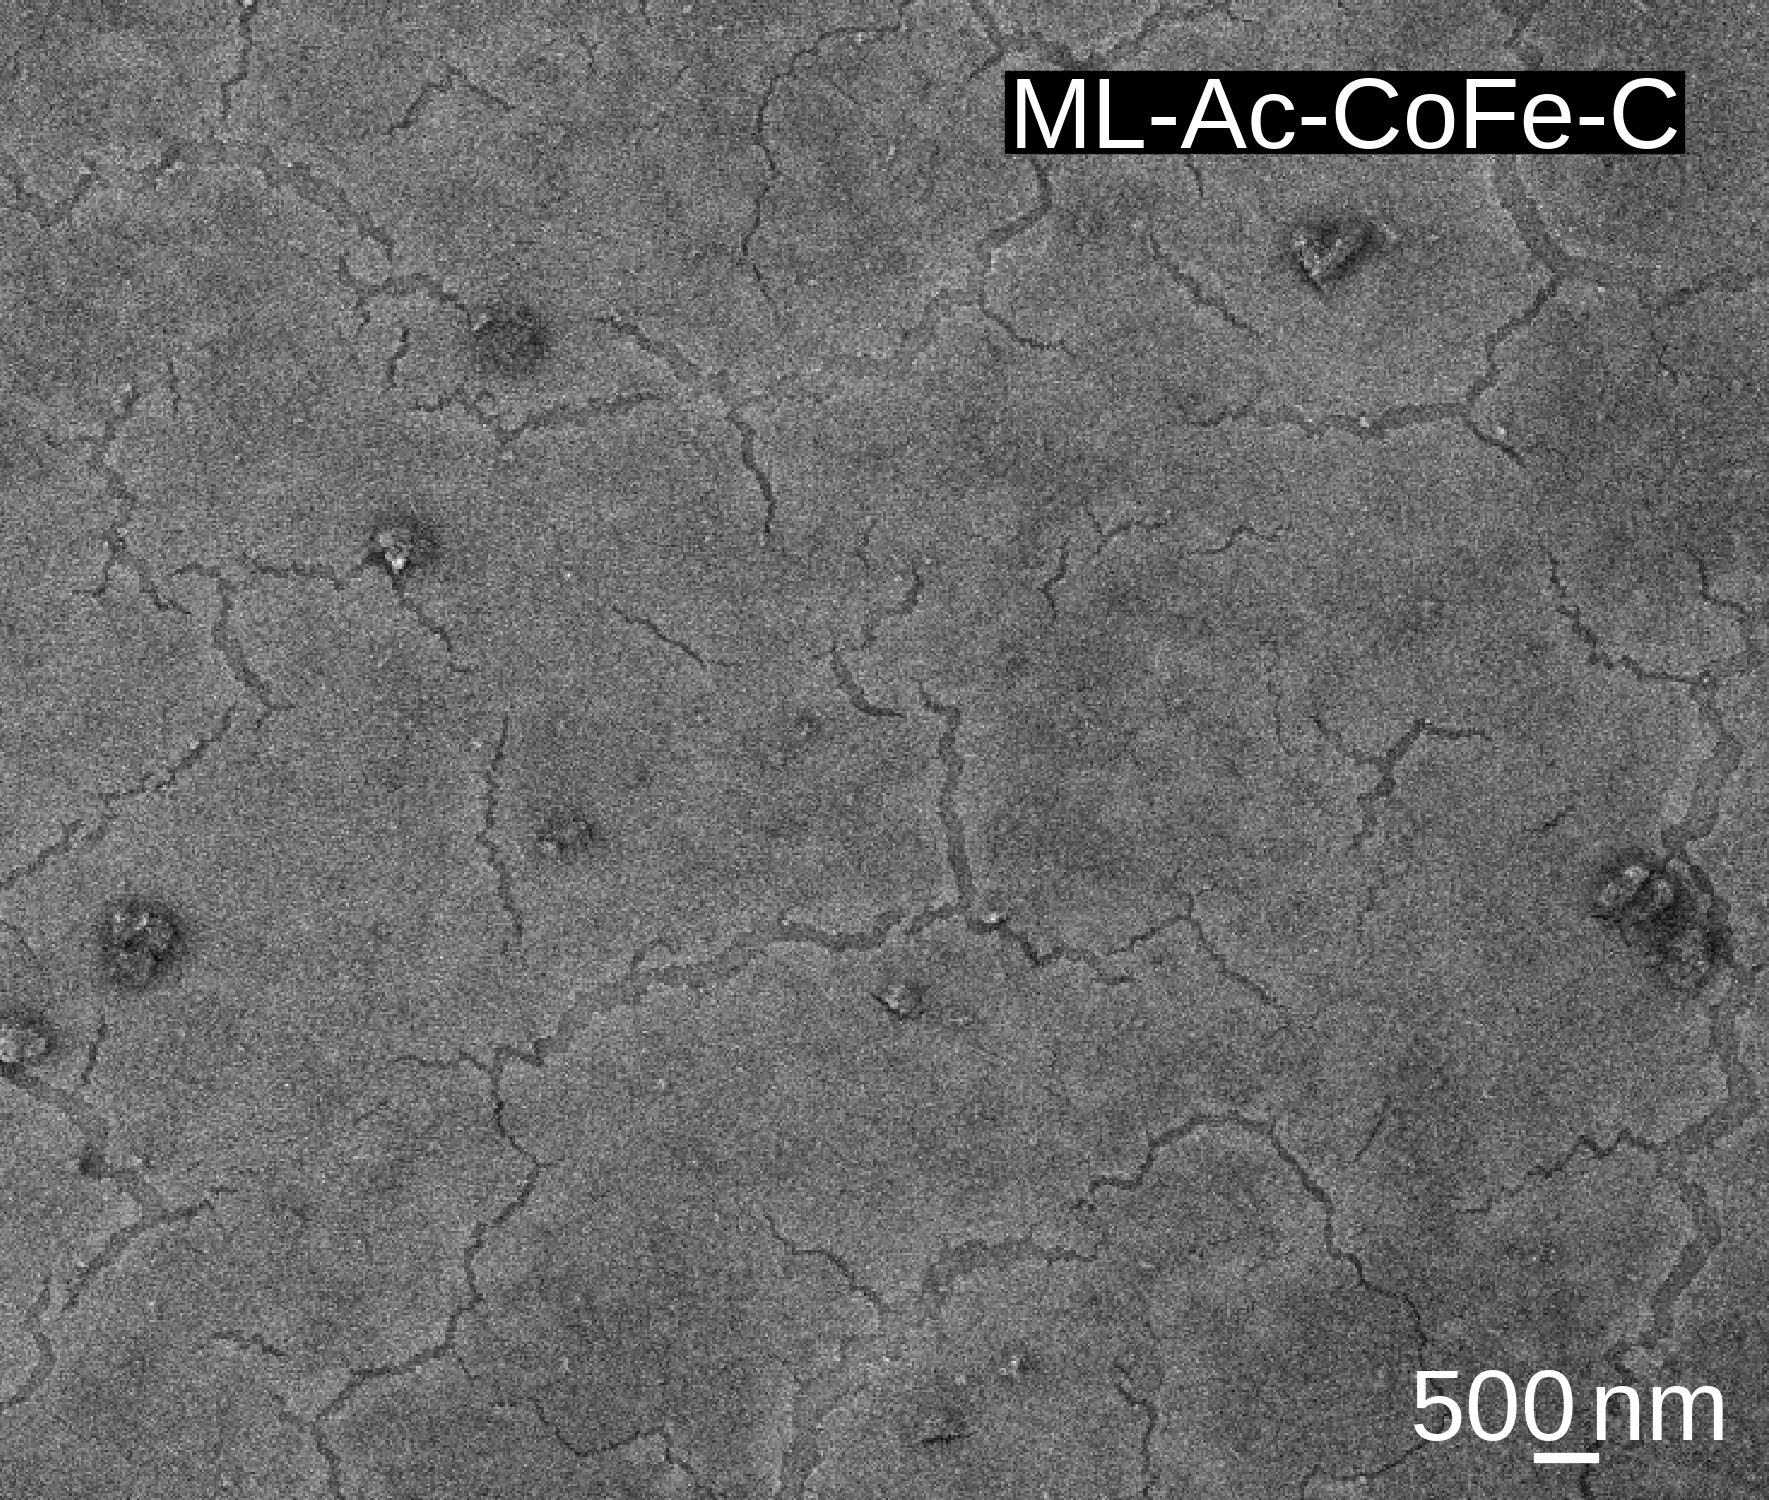
\includegraphics{monolayers_SEM_ML-Ac-CoFe-C_img1}
    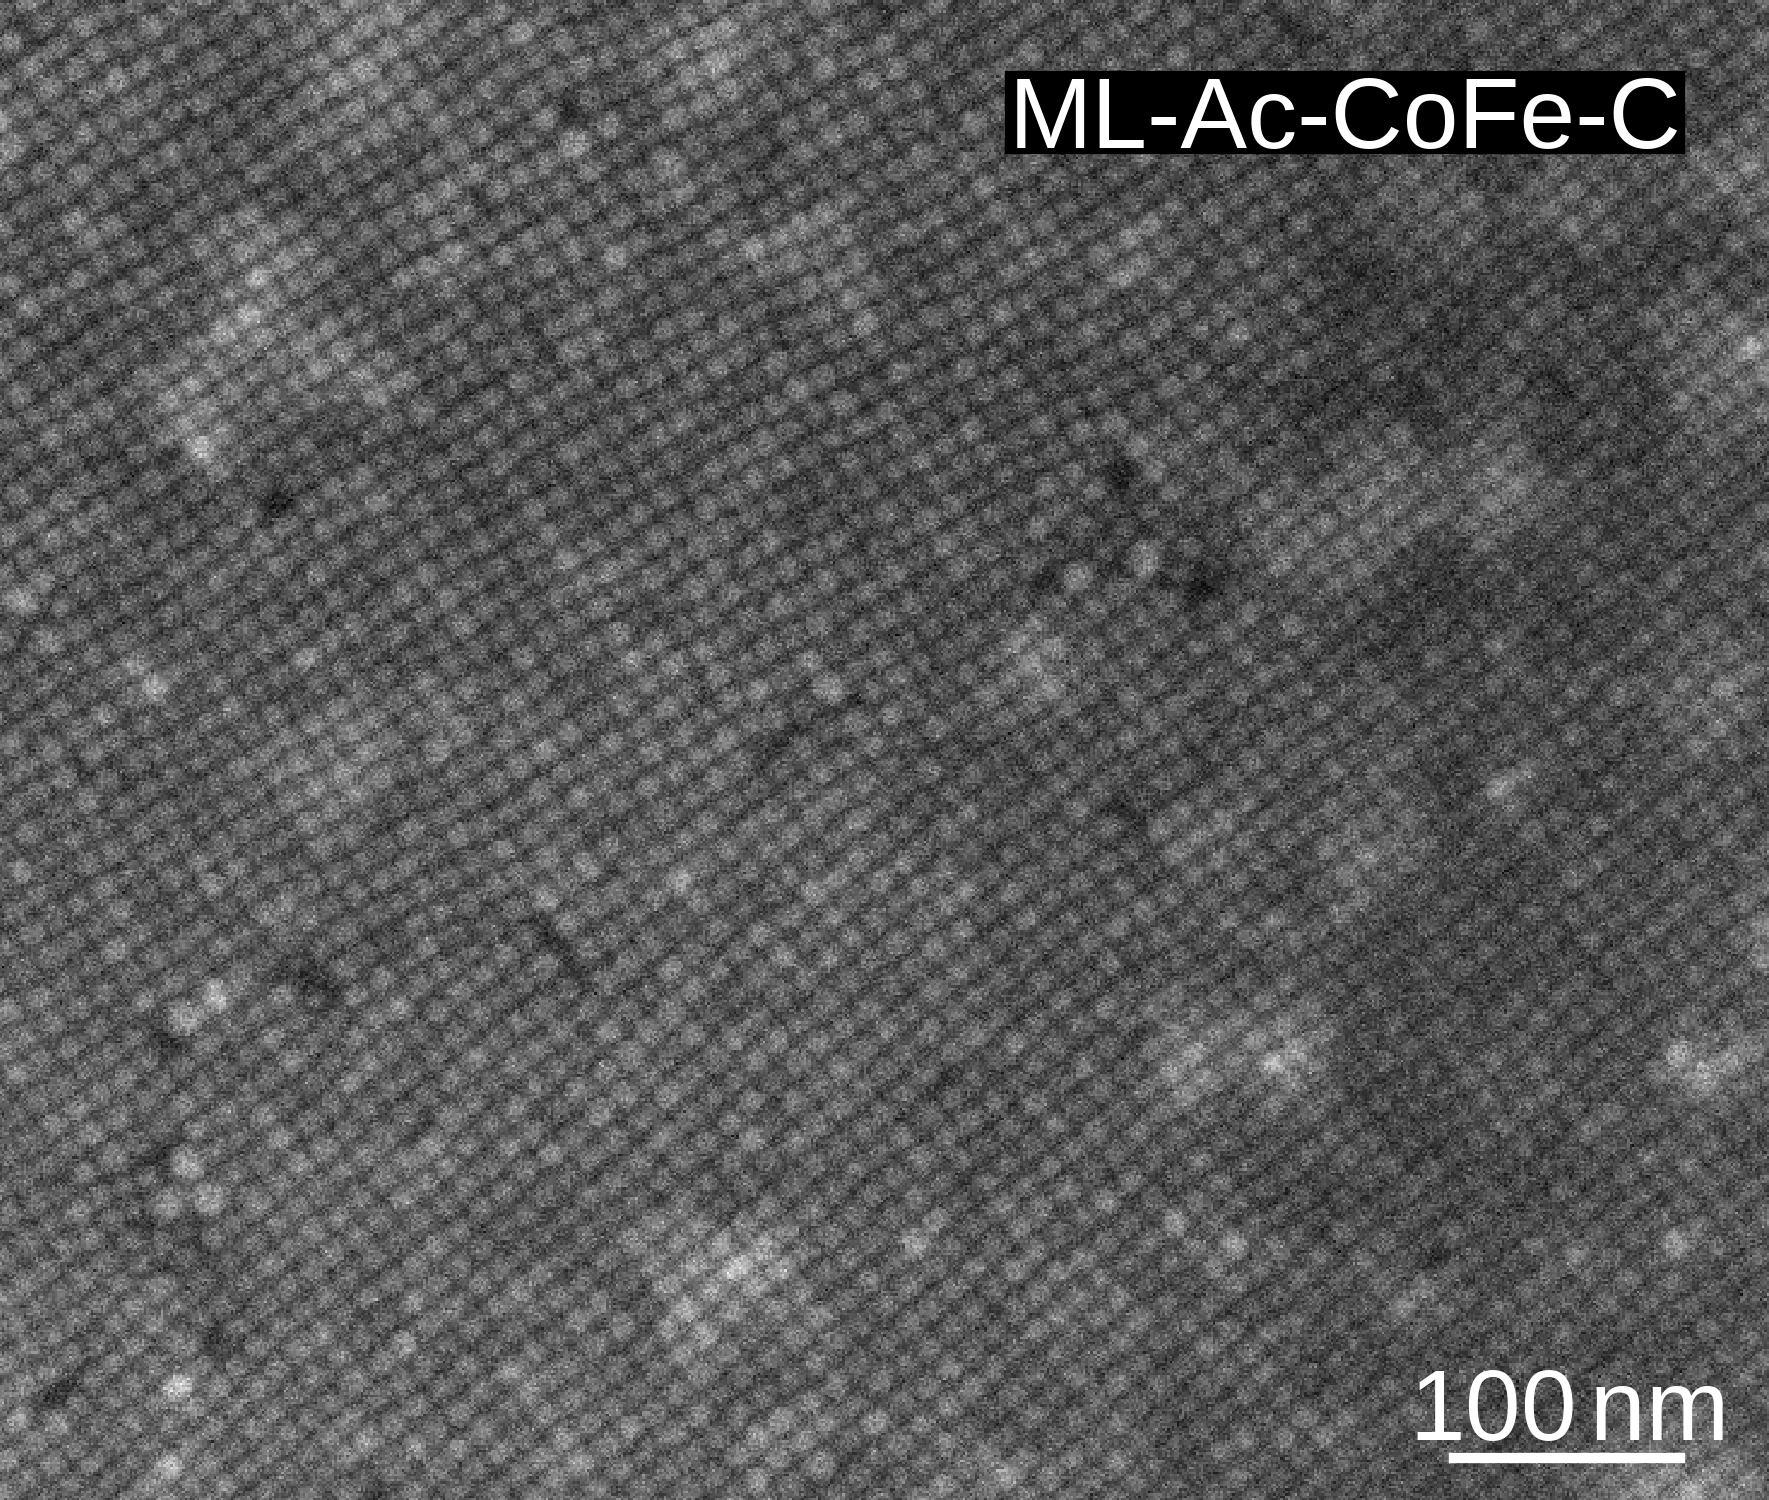
\includegraphics{monolayers_SEM_ML-Ac-CoFe-C_img2}
    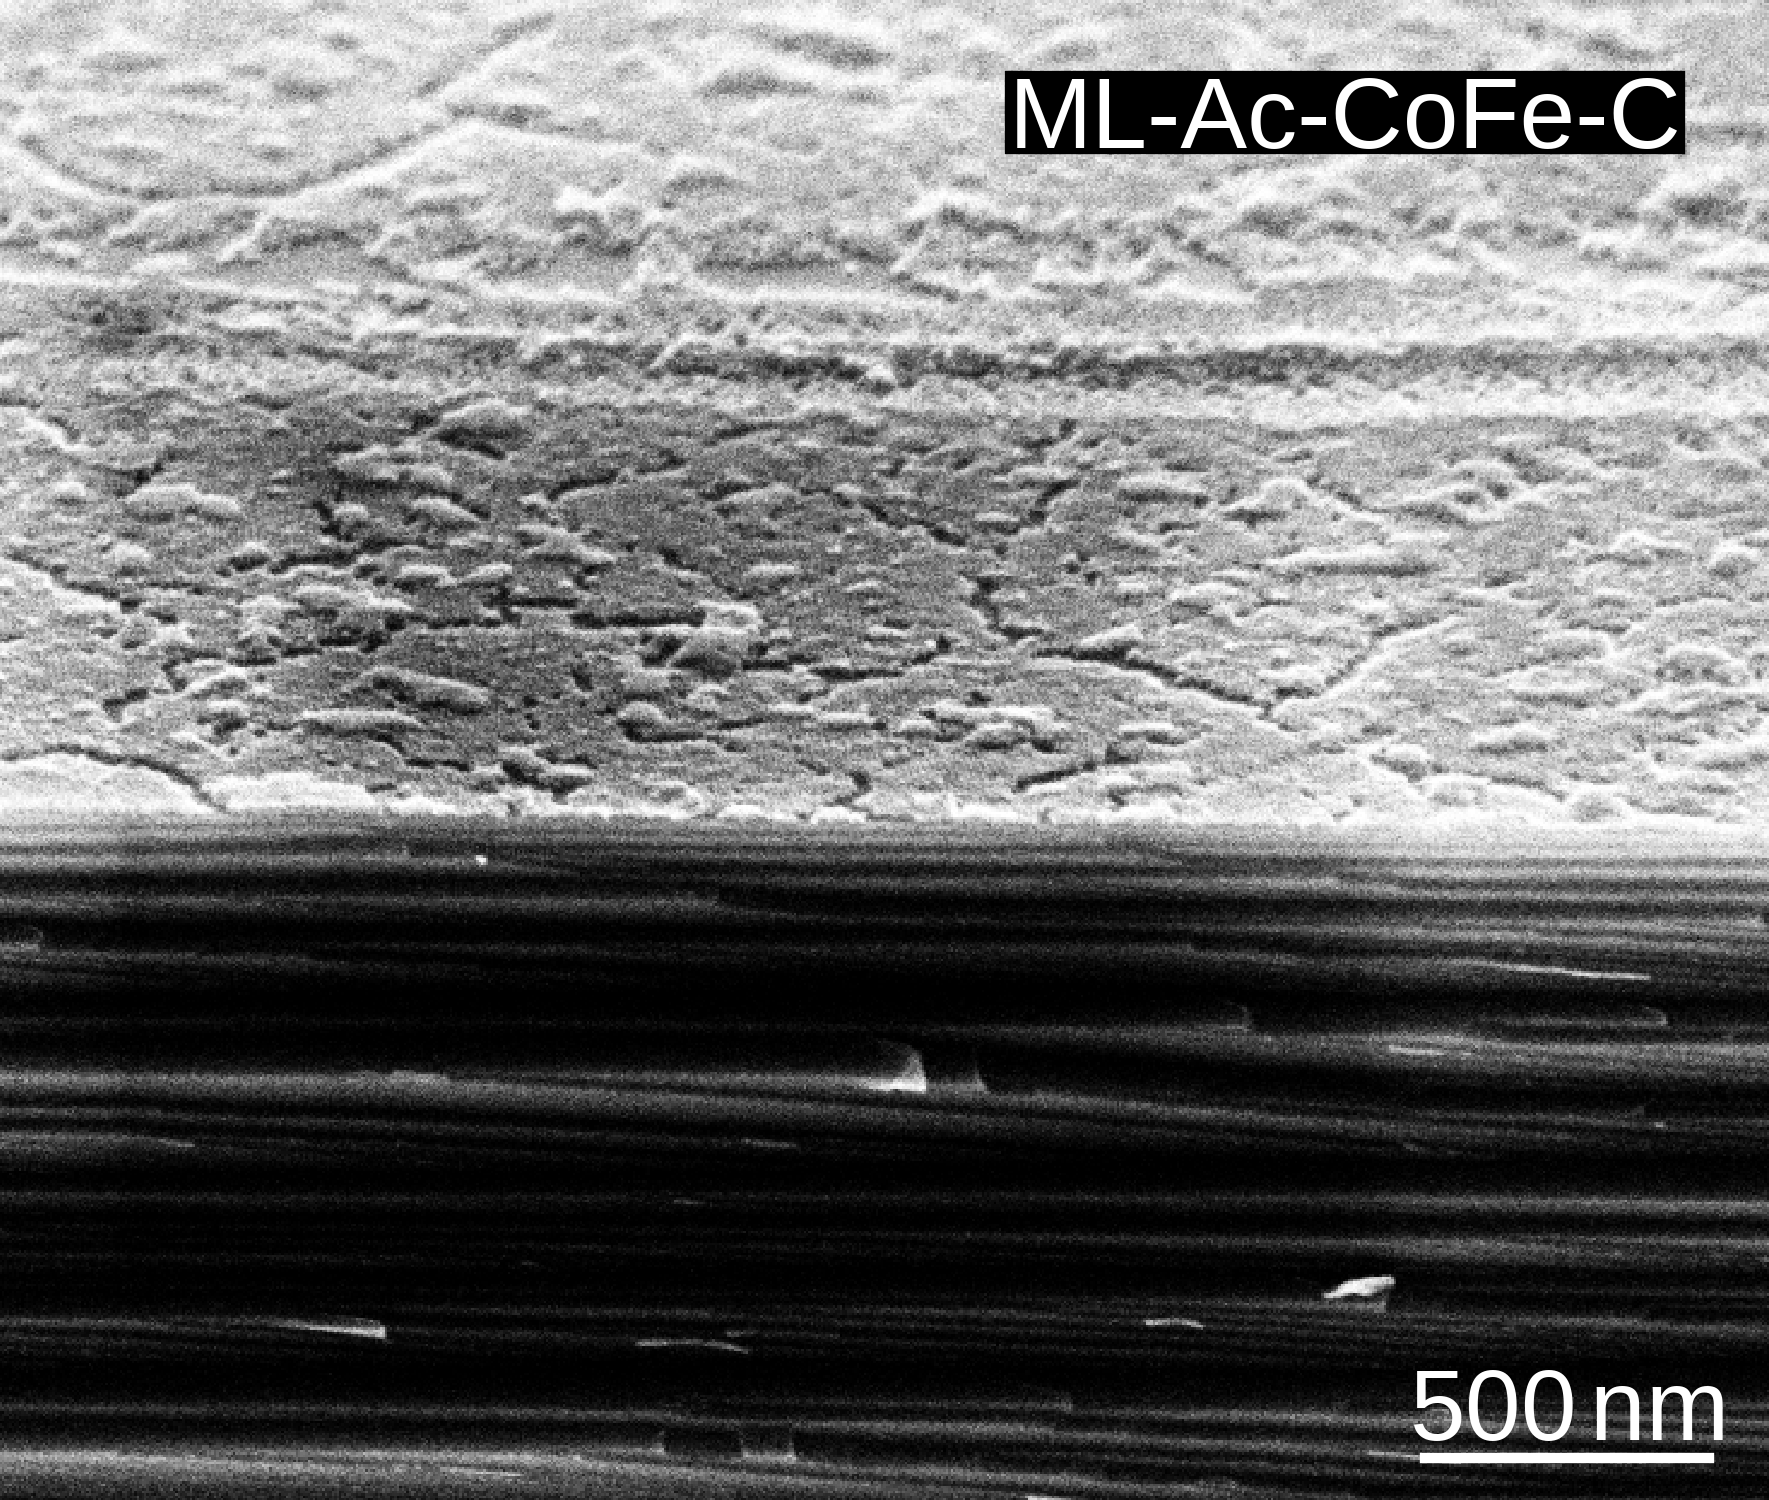
\includegraphics{monolayers_SEM_ML-Ac-CoFe-C_img3}
    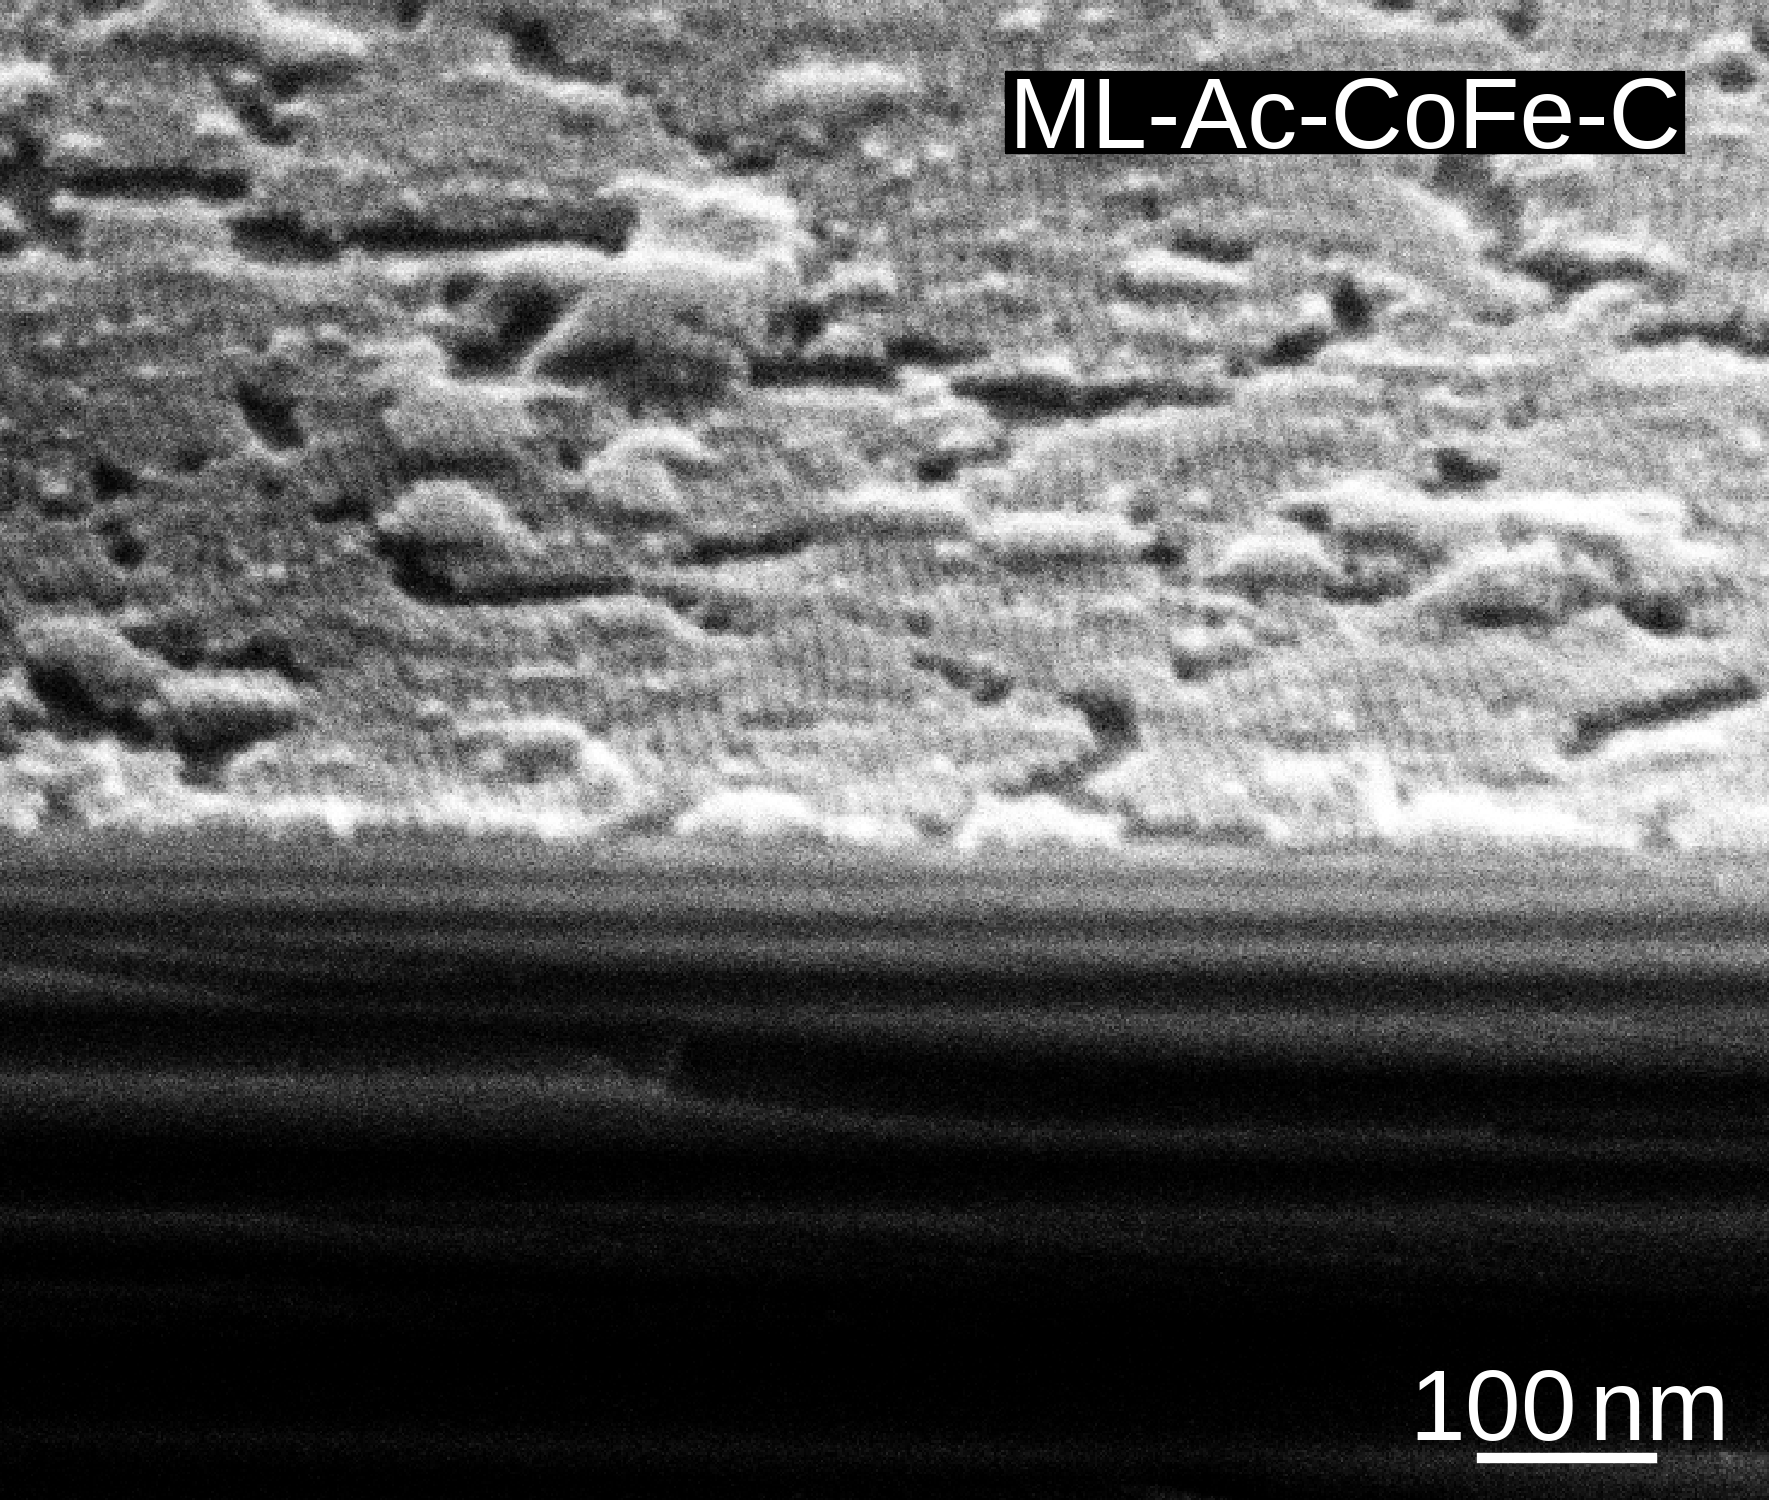
\includegraphics{monolayers_SEM_ML-Ac-CoFe-C_img4}
    \caption{\label{fig:monolayers:structure:semImagesMLACCoFeC}Micrographs of a monolayer prepared from Ac-CoFe-C-2,which is used for the study of the lateral structure of monolayers by GISAS.}
  \end{figure}

  The SEM micrographs in \reffig{fig:monolayers:structure:semImagesMLACCoFeC} locally show, the nanocubes are embedded in a square lattice arrangement and the sample has indeed a single layer structure, as visible from the cross-sectional view.
  The square array shows cracks on the length scale of a micrometer, which originate from the large size distribution of Ac-CoFe-C and it has to be noted that no additional oleic acid was added to the dispersion before drop casting as this trick was yet unknown at the point of preparation.

  The vertical structure is studied 

\end{document}